\chapter{Introduction}\label{sec1}
\epigraph{1.8in}{Los ponientes diversamente rojos que miro cada tarde serán en el recuerdo un solo poniente.}{J.L. Borges}{\textit{Historia de la eternidad}, 1936}

\section{Intonation between exemplars and abstraction}\label{sec10}
In the last century, the overwhelming majority of linguistic theories on perception of speech relied on the assumption that, in order to access meaning, listeners convert the incoming audible signal into abstract mental representations. In this perspective, which can be referred to as \textit{abstractionist}\is{abstractionism}, representations are a necessary device to cope with the extreme variability of speech productions. Variability is an intrinsic characteristic of speech: due to individual physiological differences, the same word uttered by two different speakers will be acoustically different. Even two repetitions of the same sentence uttered by a same speaker will never be exactly identical: paraphrasing Heraclitus, we could say that you cannot step twice into the same (speech) stream. 

The abstractionist approach to perception of speech has been applied to recognition and categorization of linguistic units of different levels, from activation of and discrimination among sound-based lexical representations (\textit{word recognition}) to the problems of invariance and variability of lower level units (such as syllables and segments: \textit{speech perception} proper). In both cases, it is posited that mental representations only contain ``substantial'' information, which is necessary to distinguish one representation from the other. Information which does not contribute to establishing a contrast between two representations, such as the pronunciation details discussed above (``accidental'' information, usually referred to as \textit{phonetic detail}), is not included. These simplified representations are stored in the listener's memory, and used to recognize new incoming signals. In order to perceive speech, the listener must reduce the richly detailed signal into a simplified abstract representation, by separating substantial and accidental information. This reduced representation can then be compared (and matched) with the representations which are already stored in memory. Reduction of a rich signal into a simple representation (or, in other words, separation of substantial and accidental information) is the key to generalization: to exemplify at the level of word recognition, listeners are able to recognize words produced by new unknown speakers because speaker-specific information is filtered out.

As this brief account shows, the abstractionist approach to perception of speech is strongly rooted in the linguistic, philosophical and psychological thinking which permeated the West until the first half of the last century. We avoided on purpose the use of terms such as category, feature, phonetics, phonology and normalization. But if we cast our account of the abstractionist approach into the frame of Western thinking before the 1950s, connections become visible. Focussing on word recognition, we could say that listeners map the continuously variable phonetic signal onto a discrete and abstract phonological representation, thus accessing entries in the mental lexicon. Each word in the mental lexicon is represented as the association between a meaning and a phonological form, which is in turn solely and thoroughly characterized by the contrastive features which permit to distinguish it from other forms. Entries in the mental lexicon are categories in the monothetic sense, in that they are defined by a set of singly necessary and jointly sufficient features. Perceiving speech entails the extraction of these phonological features from the signal, thus normalizing all phonetic variation. As an example, imagine that a listener is presented with the signal represented acoustically in Figure~\ref{fig101}. 

\begin{figure}
\centering
\resizebox{\linewidth}{!}{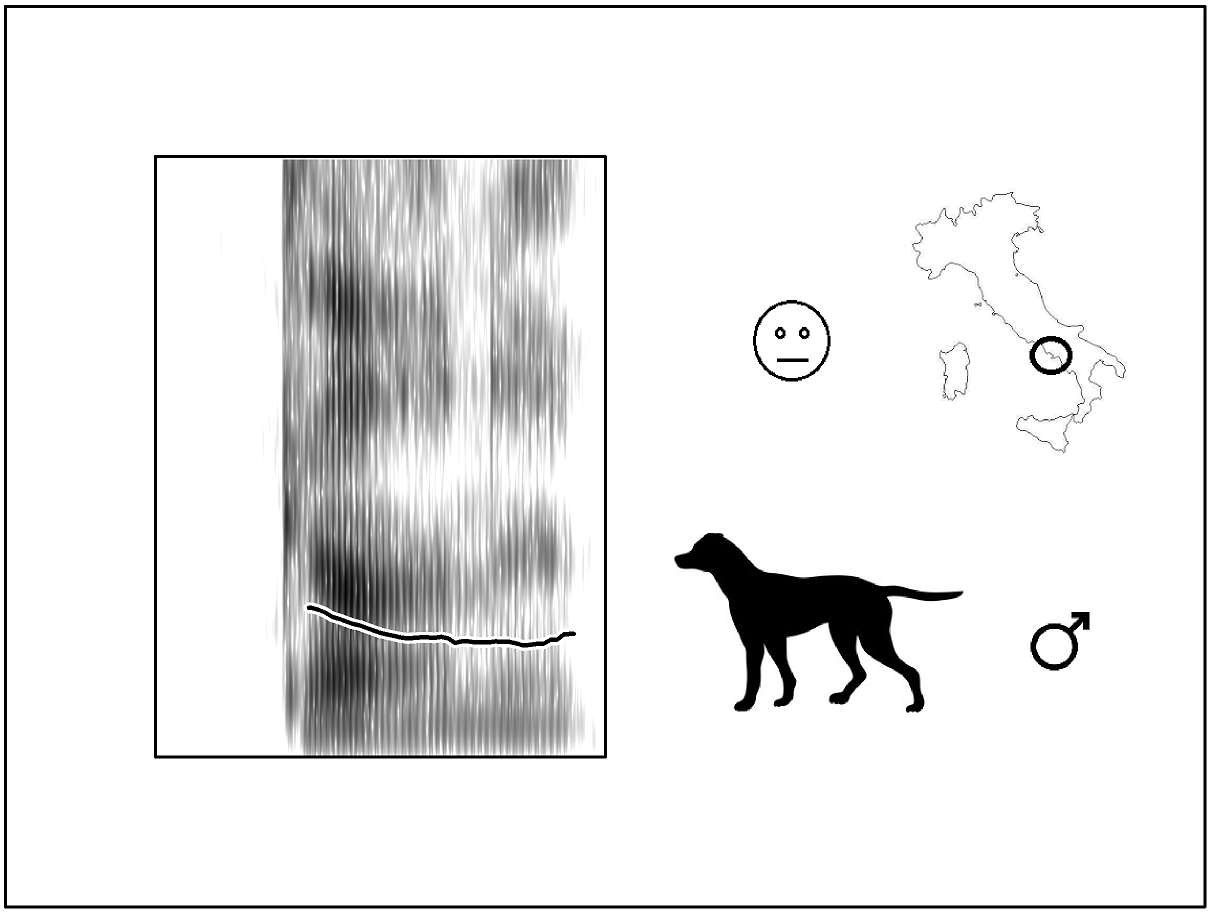
\includegraphics{images/101.png}}
\caption{Spectrogram and fundamental frequency track of the Italian word \textit{cane} `dog' as uttered by a bored male native speaker of the Neapolitan regional variety, and (part of) the information which can be extracted from the signal.}
\label{fig101}\end{figure}

According to the abstractionist approach, in the mental lexicon of Italian native speakers there is an entry, the word \textit{cane}, which links some semantic information (which we can assume to be equivalent to English `dog') with an abstract phonological form. This form is characterized by a set of singly necessary and jointly sufficient features. These could be represented by acoustical, articulatory or perceptual information, and arranged as a linear string or as a superposed score. Let us simplify on this specific point and assume they are represented by the ordered string of the phonemes /k,a,n,e/. If the actual phonetic signal is compatible with this abstract phonological representation, the word $<$cane$>$ is recognized. Crucially, in order to establish the compatibility of the phonetic signal with the phonological representation, some properties of the signal are ignored or only partially attended to. The transcription \textipa{/\textvbaraccent{}kane/} does not allow us to recover the information that the word has been uttered by a male speaker. Other features in the signal might cue other information, for example that the native variety of the speaker is the Neapolitan one. Some speakers of this variety tend to articulate low vowels with the tongue in a slightly retracted position, and final unstressed vowels are also slightly centralized. A closer phonetic transcription of the utterance above, specifying at least the position of the tongue during the vocalic portions, would thus be \textipa{[\textvbaraccent{}k\=*a:n\|x{e}]}. The signal could also be richly specified along other dimensions, such as those cueing speaker's attitudes or emotions. However, as far as word recognition is concerned, all this information must be filtered out through a normalization process. The listener will still have access to the information that the speaker is a male, that he learnt Italian in the Neapolitan area and that he is somehow bored, but word recognition will be carried on by the abstract representation \textipa{/\textvbaraccent{}kane/} alone. This representation does not contain any information which is not necessary to establish a contrast with other lexical representations. Indeed, in line with the strongly minimalist assumptions of early phonological theories, these abstract representations are as bare-boned as possible.

The idea of monothetic classes, which Western thinking inherited from Aristotle, and the clear-cut distinction between rich phonetic signal and minimalist phonological representations, which can be traced back to Trubetzkoy, represent the two pillars on which the abstractionist approach rests. However, in the last fifty years, both have been vigorously shaken by developments in philosophy, cognitive psychology and linguistics. The starting point of this renewal process can be identified in Wittgenstein's research on family resemblances\is{categorization}, which questioned in the first place the relationship between language, reality and thought, but were eventually interpreted as providing an alternative to the long-standing monothetic approach to category structure. He showed that at least some concepts are difficult (if not impossible) to define by using a finite set of singly necessary and jointly sufficient features, as in the famous example on the uses of the word \textit{game}. Some games are played for recreation, some as a profession, and some out of addiction; they can rely on muscles, brains or luck, and not all of them have scores, teams or winners. The different members of the category of games are instead linked by the propriety of sharing \textit{some} of the relevant features, none of which is necessary, and which never appear all together in any of the members.

The cognitive interpretation of Wittgenstein's investigations inaugurated a season of intense research on the structure and the formation of categories, which was mainly carried out in the 1970s by experimental psychologists working on memory and learning. The rejection of singly necessary and jointly sufficient features had major repercussions on category \textit{structure}. Monothetic categories are flat, in the sense that each member is equally representative of the class (as in the case of even numbers); categories based on family resemblances, on the other hand, have an internal structure. The members which share more features with the others are more representative (or prototypical) of the category: chess is more representative of games than Russian roulette, and robins are more representative of birds than hens. Eleanor Rosch's work on such prototypicality effects on memory and learning show how researchers' attention was shifting from abstract categories and features, as in the monothetic view, to members. The complementary line of research on category \textit{formation} went even further, by focussing on the role of concrete individual instances. The idea that categorization of a new stimulus depends on the analysis of its features and on the match with stored abstract sets of features was challenged by Lee Brooks' non-analytic approach to categorization. In his view, categorization is achieved by retrieving from memory the items which are most similar to the new stimulus. The most radical version of the main assumption behind this approach, then, is that each experience leaves an individual trace in our memory. Crucially, these traces or \textit{exemplars} are not reduced to a set of abstract and contrastive features - they rather are detailed and embodied episodes.

These developments had a deep impact on models of perception of speech. If categories are not defined by a set of singly necessary and jointly sufficient features, and if memory is a collection of individual detailed traces rather than of abstract feature sets, an exclusively abstractionist model of speech perception becomes untenable. Word recognition cannot be modelled as the result of activating a single abstract form in the mental lexicon, because storage units are detailed episodic traces. Moreover, the abstractionist approach requires, between audition and recognition, a normalization stage in which phonetic variation is separated from phonological information. And just as the postulate of monothetic classes and abstract memory was questioned by work in philosophy and cognitive psychology, recent developments in linguistics challenged the postulate of a clear-cut separation between phonetics and phonology as monolithically dealing with gradience and categoriality, respectively. Work on the interface between phonetics and phonology shows that knowledge of sound structure might rather be spread along a continuum, ranging from the fine-grained and continuous varying phonetic end, to the coarse and granular pole of lexical contrasts. By the end of the last century, then, both the psychological and linguistic assumptions behind abstractionist models were challenged.

As a result of the recent insights on episodic memory, a new approach to linguistic knowledge emerged\is{exemplarism}. Its basic principle is that linguistic categories are the result of the accumulation of individual experiences, and that linguistic structures emerge from language use. This paradigm has been applied by Joan Bybee in the study of a wide array of phonological, morphological and diachronic issues. Coupled with the insights on phonetic grounding of phonological contrasts and applied to the problems of speech perception and word recognition, this approach gave rise to a new generation of models for perception of speech, usually referred to as \textit{exemplar-based}. Models of word recognition inspired by this approach assume that listeners store phonetically detailed traces of individual events, which include both information which is necessary to lexical activation and information which concerns non-lexical contrasts, such as talker identity or context-based effects. By assuming that memory traces include detailed phonetic information, there is no longer need to account for normalization as in abstractionist approaches, and phonetic variation becomes a resource for robust categorization, rather than a source of noise for the perceptual system.

Abstractionist and exemplar-based models of perception of speech rely on a set of clearly opposed assumptions, as we tried to illustrate in the paragraphs above. However, the dichotomy between the two should not be emphasized beyond necessity. For one, exemplar models do not rule out the possibility of generating abstract representations, if only as a by-product of the activation of multiple individual traces. And abstract representations could be enriched so as to contain more phonetic information than the one exclusively required to establish phonological contrasts. Indeed, a vast amount of experimental evidence shows that both phonetic detail and abstract phonological categories play a role in speech perception and word recognition; integration of both perspectives into \textit{hybrid} models has been pursued since the beginning of the new century. The speech signal contains information at different levels of granularity, and we cannot rule out the hypothesis that insights from both approaches might be necessary to account for them all. Modelling how listeners perceive speech and handle information at different levels (e.g. lexical \textit{vs.} pragmatic contrasts), or the same information in different contexts (e.g. clear addressed speech \textit{vs.} multi-party noisy conversation), might require more than a single analytical tool. 

In order to develop a truly effective hybrid model, we should have a grasp of how linguistic information is processed along various dimensions and in various contexts. However, the striking majority of the studies informed by the abstractionist-exemplar debate deals with speech perception and word recognition alone. But words, syllables and segments do not exhaust the range of possible linguistic units. Some fifty years of intense research on prosody have shown that it is possible to find structures in the relationship between signal and meaning above the word level, as in the case of accounts on how modulations in fundamental frequency (henceforth \textit{f0}) cue contrasts on the pragmatic and informational level. If a phonological approach to intonation is possible (and even necessary, as suggested by a vast amount of evidence gathered in the last thirty years), the issue of how intonational categories are formed, accessed and instantiated must be asked as well. However, little is known about storage and retrieval of larger chunks of speech, such as phrases or entire utterances. 

In this book, we defend the thesis that the study of categoriality and gradience in intonation would benefit from insights coming from the debate on abstractionist and exemplar-based approaches to speech perception and word recognition. Our aim here is not the formalization of a model of speech perception for form-function relationships at the prosodic level. Similarly, we do not explore how chunks of speech above word level are processed, even if we recognize that these two issues would be instrumental in the development of a truly integrated hybrid model. We will rather focus on how current phonological models of intonation may benefit from research on phonetic detail, by investigating the potential role of such detail at the prosodic level (henceforth \textit{prosodic detail}) in a model of abstractionist inspiration, namely the Autosegmental-Metrical framework. Under this light, our main research question is how rich phonetic specification of phonological categories for intonation should be. Or, in other words, we question whether phonological categories in this model should be reshaped in such a way as to permit an enrichment with more phonetic information.

In the following sections, we will flesh out the title of this book, by providing our working definition of prosodic detail (Section~\ref{sec11}) and a brief account of intonation in Neapolitan Italian (Section~\ref{sec12}), the variety from which experimental data are drawn. Before turning to the experimental chapters (Sections~\ref{sec2}--\ref{sec5}), we will detail the structure of this book (Section~\ref{sec13}) and comment on some of the methodological choices overarching individual experiments.

\section{Prosodic detail}\label{sec11}
In spite of its relative recency, the concept of phonetic detail\is{phonetic detail} has already been used in a possibly confounding variety of senses. A thorough review of the history of its uses falls outside the scope of these introductory pages. However, since its exportation on the prosodic level is instrumental in setting our main research question (see Section~\ref{sec113}), we will at least provide some background and clarify our use of the term (Section~\ref{sec112}). In (Section~\ref{sec111}, we briefly review the two major shifts which characterized research on perception of speech in the second half of the twentieth century and which prepared the ground for the rise of the notion of phonetic detail: from infra-lexical to lexical units, and from abstractionist to exemplar-based approaches.

\subsection{Modelling perception of speech}\label{sec111}
Research in the relatively young field of \textit{perception of speech}\is{perception of speech} deals with how listeners represent and process speech, and how they manage to map the variability displayed by the continuous signal onto stable and discrete units \citep{jusczyk2002speech}. As we have seen above, different approaches to this main issue are possible. In abstractionist frameworks, a further line can be drawn between early work on speech perception and subsequent studies on word recognition, according to the size of the units under analysis. \textit{Speech perception} proper focusses on psychoacoustic processing of speech sounds, that is on units linking substance and form but devoid of independent function, such as segments and syllables. \textit{Word recognition}, on the other hand, deals with units associated with lexical meaning, thus focussing on activation and discrimination of lexical representations \citep{luce2003abstractness}. In the following, we argue that shifting attention from speech perception to word recognition permitted a shift in perspective from abstractionist to exemplar-based approaches. This, in turn, blurred the line between speech perception and word recognition themselves. 

\subsubsection{Speech perception}\label{sec1111}
Early studies in perception of speech were strongly influenced by the empiricism of late American structuralism and taxonomic linguistics (\citealt{harris1955phoneme, chomsky1965aspects}; see \citealt{matthews1993grammatical} for a review), which considered the observable acoustic phonetic features as the ideal starting point for a structural description of languages. In this frame, it comes as no surprise that early research on perception was mainly focussed on the phonemic level, thus equating perception of speech with speech perception. Moreover, in the late 1940s, the new spectrographic techniques started to show in full detail the acoustical complexity of speech. The alleged basic units of speech in theoretical linguistics, i.e. phonemes, were found to be highly variable.\footnote{As a result, the linguistic, phonetic and perceptual role of the segment was put under examination. Studies undermining the central role of the phoneme started with acoustic investigations on perceptual units \citep{cooper1952experiments}, progressed within Firthian and articulatory phonology in the following decades \citep{firth1948prosodies,browman1986articulatory}, and have been recast in connection with the history of writing systems already since \citet{faber1992phonemic}, and more recently by \citet{albanoleoni2006statuto} and \citet{port2006graphical}.} Phonetic variation was ascribed to two main sources, which we might label as \textit{indexical} and \textit{allophonic} \citep{luce2003abstractness} or talker variability and contextual variability \citep{johnson1997complex}, and which result in the lack of \textit{constancy} and \textit{invariance}, respectively \citep{jusczyk2002speech}. 

First, phonemes were found to have different acoustic proprieties in different segmental environments (\citealt{delattre1955acoustic}, among others). From an articulatory point of view, allophonic variation and subsequent lack of invariance in acoustic features are a natural effect of coarticulation. Sounds are not produced in strict sequentiality, but rather with a certain degree of overlap in the articulatory movements required for their production. Second, even in the same segmental environments, a given phoneme can have strikingly different phonetic realizations across talkers (\citealt{peterson1952control}, among others). Indexical variation, and the subsequent lack of constancy, are again easily understandable in an articulatory perspective, by taking into account the individual characteristics of a speaker's vocal apparatus. But even if the production of allophonic and indexical variation is motivated, what about its perception? How do listeners manage to map different acoustic proprieties to a same phonological category? As we said in the introductory pages, the problem of mapping phonetic variation onto phonological discrete categories was faced by postulating the existence of a \textit{normalization} procedure. Using either contextual \citep{ladefoged1957information} or local \citep{stevens1960model} cues, indexical and allophonic variation in the incoming phonetic signal is filtered out. 

\subsubsection{Word recognition}\label{sec1112}
The concept of normalization seemed to provide an answer to the mechanisms of speech perception, but it soon became evident that perception of speech could not be reduced to perception of consonant and vowels. For a variety of reasons, in the 1970s researchers' interest shifted from the segmental to the word level \citep{marslen1978processing}. Possible reasons for this reorientation might be traced in the advances in visual word perception (\citealt{wheeler1970processes}; see \citealt{balota1994visual} for a review), or in the ever growing interest of the linguistic research community in syntactic structures, which are instantiated by words. More probably, it is the intuitiveness of the link between form and meaning at the word level that turned words into the main research object, since it provided a bridge between sound and sense, thus allowing the extension of perception into understanding.\footnote{Limitations to the role of features and segments as central level of progressing also came, for example, by studies on the understandability of spectrally rotated speech \citep{blesser1972speech}.} This allowed research on word recognition to join ends with issues in how memory storage works, through the notion of mental lexicon \citep{oldfield1966things}.

Different comprehensive models of spoken word recognition appeared in the 1980s, such as \textit{Cohort} \citep{marslen1980temporal} and \textit{Trace} \citep{mcclelland1986trace}. We will not detail here the structure of these models, which moreover have been (in some cases thoroughly) revised in the last years. What is relevant to our discussion is that they both share the assumption that word recognition is mediated by primitive sub-lexical units (phonemes in \textit{Cohort}, features and phonemes in \textit{Trace}), thus qualifying as abstractionist models of word recognition. Abstractionist approaches assume, at various degrees of explicitness,\footnote{See \citet{licklider1952process, peterson1952information, lindgren1965machine}. According to \citet{luce2005spoken}, with the exception of \citeauthor{klatt1979speech}'s \citeyearpar{klatt1979speech} model of \textit{Lexical Access From Spectra}, virtually all current models of spoken word recognition are based on abstractionist assumptions. Accounts of visual word recognition based on distributed models of memory \citep{mcclelland1985distributed} are labelled by \citet{tenpenny1995abstractionist} as \textit{weakly episodic}; this however does not diminish the role of sub-lexical units in \textit{Trace}, on which we base our conclusions.} that words are represented as separate, abstract and idealized ``types'' in the mental lexicon, using conventional abstract representational formats built of discrete abstract features or phonemes.

\subsubsection{Exemplar-based models}\label{sec1113}
As we have seen in the introductory pages, on the other hand, according to exemplar theories\is{exemplarism} the lexicon is built by a myriad of phonetically detailed traces, one for every ``token'' of spoken words, which are formed as words are repeatedly encountered by the listener in her life-long experience.\footnote{Accepting that every single experience leaves an individual trace entails assuming that storage capacity for human memory is virtually unlimited. Proponents of exemplar-based approaches cite findings from \citet{standing1970perception}, showing that subject have surprisingly accurate recall rates (above 90\%) of vast amounts of pictures (more than 2500) even with short presentation times (down to 1s) and long test times (3 days). Another line is to assume some kind of information reduction, as in the \textit{Alcove} connectionist exemplar model \citep{kruschke1992alcove}.} Exemplar-based approaches to perception of speech are not restricted to word recognition, as \citeauthor{johnson1997speech}'s \citeyearpar{johnson1997speech} early work on vowel perception shows. However, the shift from speech perception to word recognition that we discussed in the previous subsection permitted an easier percolation of new ideas from neighbouring fields. Research on visual word recognition \citep{tenpenny1995abstractionist}, in fact, had already assimilated insights from non-analytic cognition \citep{brooks1978nonanalytic} and  early modelling of episodic memory \citep{medin1978context}. Studies on the computational implementation of this approach flourished in the following decade \citep{mcclelland1981retrieving, hintzman1986schema, nosofsky1986attention}, and provided in the 1990s a testing ground for exemplar approaches to perception of speech.

The first studies in this direction focussed on memorization of voice in isolated words \citep{goldinger1991nature,schacter1992auditory,palmeri1993episodic,church1994perceptual,goldinger1996words}. Both explicit (recall) and implicit (priming) memory were tested using both clear and degraded (low-filtered) speech. They found facilitatory effects of known voices, which were accounted for by assuming storage of phonetic information relative to talker identity. That is, against the abstractionist assumptions, indexical variation is retained and participates in word recognition. Exemplar-based explicit models were used by \citet{johnson1997speech} to simulate, among others, identification of different vowels across various speakers. Each stored exemplar consisted in vowels extracted from read words and reduced to a set of acoustic features (fundamental frequency, first three formants, duration) linked to a set of category labels (the intended word, the sex and the identity of the speaker).\footnote{Following \citet{nosofsky1988exemplar}, stored exemplars are activated on the basis of acoustic similarity with the incoming signal. Similarity is calculated using attention weight and euclidean distances between values of the acoustic features. Activation of exemplars, in turn, yields evidence for the category labels they are associated with, ultimately leading to classification.} The high correct identification rates show that an exemplar-based model can use indexical variation as a resource for speech perception, thus circumventing the need for normalization procedures.

If indexical detail is included in episodic memory traces, words can be accessed without normalization of sub-lexical units. Words are stored as connections between category labels and detailed acoustic traces, and not as abstract strings of segments. Thus there is no need to recover abstract segments from the signal in order to access the higher level of word processing. In this sense, exemplar-based models suppress the modularity between speech perception and word recognition which is posited by abstractionist models. However, as we suggested at the beginning of this section following \citet{luce2003abstractness}, abstract representations filter not only indexical (speaker-dependent) details, but also allophonic (context-dependent) phonetic information. In exemplar-based models, indexical and allophonic variation is handled without substantial differences. The distinction is however crucial in abstractionist approaches, since the treatment of allophonic detail is strictly related to the construction of phonological categories. We take up this issue in the next section.

\subsection{Phonetic detail}\label{sec112}\is{phonetic detail}
Unlike indexical or speaker-specific variation, treatment of allophonic or context-based variation has always been a core issue in phonology. Inspired by the saussurean emphasis on the differential function of elements within a system, early structuralist phonology stressed paradigmatic relations in the individuation of units. That is, phonemes were intimately linked to the notions of distinctiveness and contrast. The paradigmatic dimension was seen as constitutive, but syntagmatic aspects (pertaining to the linear combination of units) were not excluded from the scope of phonology. Since its structural origins, phonology dealt with both contrast and distribution, with both archiphonemes and, crucially, allophones. This long-term acquaintance with syntagmatic and context-based processes might explain why, when exemplar-based models of perception suggested new ways of handling allophonic and indexical variation, allophonic variation received the greatest share of interest in the linguistic research community. Much of the recent studies on the so-called \textit{(fine) phonetic detail} deal in fact with phonetic information linked to language-specific rather than speaker-dependent variation. In a very broad sense, phonetic detail could be defined as systematic phonetic variation excluded from abstract phonological representations. 

\subsubsection{Context beyond phonemes in word recognition}\label{sec1121}
By qualifying this variation as \textit{systematic}, we draw a line between language-specific and speaker-dependent variation, as we said above, thus excluding indexical variation from our definition of phonetic detail. However, this does not mean equating phonetic detail with allophonic variability in the sense of \citet{luce2003abstractness}. As they put it, quoting \citet{ladefoged2000course}, allophonic variation refers to context-induced articulatory and acoustic differences among speech sounds belonging to the same phonemic category. But this definition is only viable when focussing on speech perception and word recognition - that is, when the only functional contrasts under examination are those based on phonemic categories, thus at the lexical level. Decades of research on the structures of conversation, talk-in-interaction and prosody, however, have convincingly shown that ``meaning is much more than lexical meaning'' \citep{local2003variable}. In this sense, perception of speech does not boil down to accessing meaning through the mental lexicon. Crucially to our discussion, then, context-induced phonetic variation should not be exclusively sought at the phonemic level (allophonic variation), but at all levels of granularity in form and substance, with respect to all systematic functional variation (phonetic detail). 

A review of the possible roles of phonetic detail is provided by \citet[§5.1]{hawkins2003roles}. Such phonetic information is systematically produced and, at least ``in the right circumstances'' \citep{hawkins2010phonetic} as in the case of adverse listening conditions, used as a cue to the perception of various contrasts. Systematic phonetic variation might cue word boundary placement: [s] duration and possibly degree of diphthongization of the second nucleus help listeners in segmenting the phoneme string \textipa{/katsaIz/} as \textit{cat's eyes} or \textit{cat size} \citep{hawkins2001polysp}. Differences in periodicity, aperiodicity and voice onset time ratios systematically distinguish prefixes and pseudo-prefixes, as in \textit{discover} versus \textit{discolour} \citep{smith2012phonetic}. Variations in speech rate and in articulatory tension provide a set of devices for turn management (see \citealt{local2003phonetics} for a review). Apart from localized phonetic information cueing non-segmental contrasts, phonetic detail might also refer to segmental contrasts cued by diffuse phonetic information. This is the case for the so-called short and long domain r-resonances in English: acoustic differences between pairs like \textit{miller} versus \textit{mirror} are not exclusively localized in the intervocalic portion \citep{kelly1986long}. Moreover, when the intervocalic portion is masked by noise, listeners still manage to make reliable identification judgments \citep{west1999perception,heinrich2010influence}. Diffuse cues are not restricted to r-resonances: see \citet{hawkins2004influence} on voicing of coda obstruents and \citet{coleman2003discovering} on the feature [anterior]. Phonetic detail might also be linked with frequency of use, as in the case of differences in duration of post-stress schwa before non-wordfinal non-labial sonorants. Words with increasing frequency like \textit{mammary}, \textit{memory} or \textit{every}, thus tend to have progressively shorter schwas \citep{bybee2001phonology}.\footnote{See \citet{hooper1976word} for a use of ``schwa deletion'' (the binary version of the durational differences reported above) in the perspective of frequency-based morphophonological change. For a recent review on frequency-based ``acoustic reduction'', see \citet{ernestusacoustic}.}

Phonetic detail thus encompasses this broader spectre of phenomena, by relying on an extended vision of allophony, affecting both the definition of context (beyond adjacent phonemes on the segmental string) and domains within perception of speech (beyond lexical meaning in word recognition).

\subsubsection{Present exclusion from phonological representations}\label{sec1122}
As we suggested in our definition above, this systematic variation must be \textit{excluded} from abstract phonological representations in order to qualify as phonetic detail. The use of a negative definition here should not be mistaken for a theoretical weakness. On the contrary, it has the advantage of suggesting a strict link between our current understanding of phonetic detail and the debate from which it originates. As such, negative features are present in virtually all definitions of phonetic detail (or fine phonetic detail, FPD): for example, ``the term FPD has come to be applied to anything that is not considered a major, usually local, perceptual cue for phonemic contrasts in the citation forms of lexical items'' \citep{hawkins2010phonetic}, or ``FPD refers to phonetic properties that are judged non-essential in the identification of speech sounds in a theoretical framework whose limits the exemplar approach endeavors to demonstrate'' \citep{nguyen2009dynamical}. As a result, phonetic detail does not exist in its own right, but only as a mirror reflecting a particular thread of evolution in linguistic thinking: we call phonetic detail all phonetic information which \textit{has been} treated as (negligible) detail in abstractionist approaches, but which \textit{is now} treated as (possibly) useful information in exemplar-based approaches. 

Let us push the intrinsic historicity of phonetic detail to its extremes. As we said above, we are looking for phonetic information which can be recognized as useful once we move from an abstractionist to an exemplar-based approach. This leaves us with the issue of phonetic information which has already been recognized as systematic and useful within \textit{abstractionist}\is{abstractionism} approaches themselves. To exemplify, the essential phonetic exponents of the phonological contrast in voicing \citep{trubeckoj1939grundzuege} have initially been identified in vocal fold vibration and low frequency periodicity \citep{jakobson1952preliminaries}, on the articulatory and acoustic dimensions, respectively. Focussing on the acoustic dimension and on non-final stops, we could say that at this stage the phonological contrast between voiced and unvoiced is cued by presence or absence of periodicity during closure. However, the exploration of the voicing contrast across different languages \citep{lisker1964crosslanguage}\footnote{Languages with three-way stop contrasts were instrumental in drawing researchers' attention on cues other than periodicity during closure. Voice onset time, for example, received perhaps its first formalization in early work on Armenian dialects \citep{adjarian1899explosives}.} eventually led to the discovery of a great number of systematically produced and perceived acoustic cues to voicing contrasts \citep{lisker1986voicing}. If we do not usually consider voice onset time as an example of phonetic detail,\footnote{On this topic, see also \citet{vanalphen2006effect}. For studies on indexical aspects of voice onset time in an exemplar-based perspective, see \citet{theodore2009characteristics} and \citet{levi2010priming} instead. However, as we argued at the beginning of this subsection, we are now focussing on (extended) allophonic aspects.} it is because it has already been accommodated inside abstractionist approaches to speech perception. This has been done by \textit{enriching} the representation of the phonological contrast in voicing for a given language with phonetic information beyond periodicity during the closure. 

As we said above (see Section~\ref{sec111}), abstractionist and exemplar models crucially differ in the degree of phonetic information stored in mental representations. However, finding new systematically produced and perceived phonetic information does not constitute an evidence for the inadequacy of abstractionist approach altogether - it does not prove that abstraction plays no role in perception of speech. At best, discovering new phonetic detail can be seen as evidence for the inadequacy of \textit{currently available} abstractionist models. As we have seen in the introductory pages, the sharp divide between bony phonological categories and rich phonetic signal is not an indisputable matter of fact, but rather a theoretical heritage of early structuralism. As such, it can be questioned when new findings are made available, and in the last years it has indeed been questioned by new developments in phonology.\footnote{Work in laboratory phonology \citep{ohala1990interface,pierrehumbert1990phonological,pierrehumbert2000conceptual} and inspired by optimality theory \citep{flemming1997phonetic,flemming2001scalar} are perhaps the best examples of these new developments.} In this sense, the notion of phonetic detail has the merit of fostering research from both abstractionist and exemplar-based perspectives. As \citet{nguyen2009dynamical} point out, sensitivity to phonetic detail is not inconsistent with abstractionist models which allow for richer phonological representation, as in the case of \citeauthor{stevens2004invariance}' \citeyearpar{stevens2004invariance} language-specific enhancing gestures or of \textit{Trace}'s interactive account of fine-grained coarticulatory variation \citep{elman1988cognitive}. Exemplar-based approaches provide an intrinsic account for the role of phonetic detail, since they assume that all phonetic information is stored in long term memory. Abstractionist approaches, on the other hand, must review the early assumption of minimalism in phonological categories, and permit an \textit{enrichment} with phonetic information previously dismissed as meaningless or predictable variation.

\subsection{Prosodic detail}\label{sec113}\is{prosodic detail}
From an abstractionist perspective, phonetic detail thus offers a vantage point to explore the relationships between phonetics and phonology. It points to the need of including more phonetic information in phonological representations. But if we see the glass half full, once phonological representations are properly enriched, phonetic detail might even represent evidence for abstraction mechanisms themselves. That is, phonetic detail might point to the need of rich abstract representations, meaning that we need both the enrichment \textit{and} the existence of abstract representations. In the following we exemplify this dynamics by focussing on intonation. We discuss how the exploration of phonetic detail at the prosodic level, while apparently providing evidence against phonological approaches to intonation, could actually lead to their validation and refinement.

As we said above, exemplar-based models posit storage of phonetically detailed traces in long term memory. Phonetic details at the word level, such as r-resonances \citep{heinrich2010influence}, voicing of coda obstruents  \citep{hawkins2004influence} and durational patterns in prefixed and pseudo-prefixed words \citep{smith2012phonetic}, are stored in the individual acoustic traces associated with those exemplars. We have seen that storage of individual traces at the word level entails virtually unlimited memory capacity. But what about phonetic detail spanning above word level and functioning as cue to non-lexical contrasts, as in the case of variations in speech rate and articulatory tension as devices for turn management \citep{local2003phonetics}? Should we conclude that memory provides storage for entire utterances as well? In this case, the ``head-filling-up problem'' \citep{johnson1997speech} would become simply unsolvable.\footnote{More importantly, positing memory storage for entire utterances would ultimately mean dismissing the whole lexicon-grammar duality, and pulverizing both paradigmatic and syntagmatic dimensions in a myriad of isolated points. Even exemplar-based approaches to grammar as emergent structure refuse to venture this far \citep{bybee2001phonology}.}

\subsubsection{An alternative to phonology}\label{sec1131}
Exemplar-based approaches do however allow plausible storage of information beyond words and lexical meaning. First, we could not exclude processing and storage as single units of particular chunks above word level, as in the case of idioms (such as \textit{pull strings}) and collocations (such as \textit{prominent role}) \citep{bybee2006usage}. And more importantly to our discussion, since exemplars are supposed to include all sort of detailed phonetic information, they could indeed include not only temporal and spectral information useful in accessing lexical meaning, but also melodic information useful in accessing post-lexical meaning. That is, stored exemplars might contain as well time-aligned fundamental frequency contours, and exemplars of a same word with different f0 information might be linked to different categorical labels referring to informational and pragmatic meaning. Recent research on the effects of word frequency on variability in the production of pitch accents is indeed aimed at verifying this hypothesis \citep{walsh2008examining,schweitzer2009frequency,schweitzer2010frequency}, and will be extensively reviewed and commented in the concluding remarks (see Section~\ref{sec63}). 

With regard to our present discussion, the strongest form of the theoretical implication behind these studies is the rejection of \textit{post-lexical accounts of prosody}\is{exemplar prosody} assignment \citep{schweitzer2010relative,schweitzer2011prosodic}.\footnote{More precisely, the authors question the usual assumptions according to which ``prosody is `post-lexical' in English'' \citep[1]{schweitzer2011prosodic}, ``prosody is assigned `post-lexically' in English'' (ibidem) and ``accenting is `post-lexical' in English'' \citep[1]{schweitzer2010relative}, meaning that ``prosodic realisation is determined
by a combination of `top-down' syntactic, semantic and pragmatic factors (e.g. given/new status), and the phonological context (e.g. how close together accents are)'' \citep[4]{schweitzer2011prosodic}. If \textit{post} in post-lexical is not intended in terms of sequential application of generative transformational rules, we could say that by rejecting post-lexical accounts of prosody the authors essentially question \citeauthor{beckman1996parsing}'s \citeyearpar{beckman1996parsing} claim that prosody is a grammatical structure to be parsed.}  If not all, most accounts of the relationships between sentence-level meaning (e.g. syntactic chunking, information structure, pragmatic meaning) and phonetic information (mainly fundamental frequency, duration and amplitude) rely on the assumption that the prosodic component in general and intonation in particular can be somehow separated from the lexical material which composes a given utterance, at least on a descriptive level. This assumption is central in those approaches emphasizing the role of phonological structures in prosody \citep{ladd2008intonational}. The best example is provided by the notion of the independence between tune and text, which permeated from \citet{liberman1979intonational} through \citet{pierrehumbert1980phonology} into modern AM approaches to intonation (see Section~\ref{sec122}).\footnote{According to which ``tunes are linguistic entities, which have independent identity from the text. Tunes and texts cooccur because tunes are lined up with texts by linguistic rules'' \citep[19]{pierrehumbert1980phonology}.} However, even in approaches which do not posit the existence of phonological structures in intonation and suggest a direct link between phonetic exponents and sentence-level meaning (a line of research that goes from \citealt{cooper1980syntax} to \citealt{xu2005speech}), or even more so in the so-called superpositional models of intonation (e.g. \citealt{fujisaki1982modelling}), intonation is seen as somehow orthogonal to lexical material. 

Thus, \textit{both} phonological and phonetic approaches to intonation can posit a post-lexical assignment of prosody. On the other hand, negation is not a symmetrical function in this case: exemplar-based models which reject post-lexical assignment of prosody can \textit{only} allow for a phonetic approach to intonation. If we assume that f0 contours are stored as part of the phonetic information of a given exemplar, and directly linked to categorical labels of informational and pragmatic meaning, we can dismiss altogether the notion of an abstract and discretized level of representation for intonation. There is no longer need for independent and abstract tunes, composed by pitch accents and boundary tones, and embodied in the actual text of an utterance. When a listener is presented with a word, a part of its phonetic information (especially the spectral one) will activate lexical meaning, and another part (especially the melodic) will activate post-lexical meaning. In both cases, for phonemes as for pitch accents, abstractions would be at best a by-product of exemplar activation. 

\subsubsection{A resource for phonology}\label{sec1132}
However, evidence of structures in intonation and thus support for phonological approaches have become overwhelming in the last thirty years (see \citealt[§1.3 for a review]{ladd2008intonational}). In suggesting the existence of a direct bridge between phonetic information and sentence-level meaning, exemplar-based approaches to prosody might actually represent a step backwards. This does not mean that research on prosodic detail is altogether incompatible with phonological approaches to intonation. As we said above, the intrinsic historicity of the notion of phonetic detail leaves open the possibility of refining abstractionist approaches as well (see Section~\ref{sec112}). By enriching our phonological representation of voicing contrasts, for example, allophonic variation in voice onset time can also be framed in abstractionist terms, without the need of dispensing from the ideas of linearity and discreteness. Acknowledging the existence of multiple phonetic cues to a given phonological contrast has indeed been instrumental in the formulation of new research questions, such as in the investigation of trading relationships between perceptual cues (e.g. \citealt{repp1979relative}). Before dismissing abstractionist assumptions altogether, we might well want to push them to their limits, and see whether they lead to new and possibly interesting research questions.

This is precisely the spirit which animates this book. In the following chapters, we will explore how the study of prosodic detail might be useful in reshaping phonological representations for intonation. Unlike the literature on exemplar prosody we reviewed in the subsection above, we start from the assumption that it is both possible and necessary to posit the existence of abstract phonological structures in the study of intonation. For this reason, we will frame our experiments in an overtly abstractionist model of intonation, the Autosegmental-Metrical framework (see Section~\ref{sec12}). By gathering evidence on prosodic detail on both the melodic and temporal dimension, we will question some of the strictly minimalist assumptions behind this model, and suggest some improvement strategies where necessary. Our purpose, however, is neither to develop a new abstractionist model of intonation, nor to rule out the viability of alternative exemplar-based approaches. We rather aim at showing how research on phonetic detail at the prosodic level might be a resource in the exploration of the relationships between phonetics and phonology.

\section{Neapolitan Italian intonation}\label{sec12}
If prosodic detail is language-specific systematic phonetic variation excluded from phonological representations in current abstractionist intonational models, its exploration requires the choice of at least one language and one model of intonation. In this section we provide some basic information on both the variety we draw our data from, Neapolitan Italian (henceforth \textit{NI}\is{Neapolitan Italian}; see Section~\ref{sec121}), and the framework we use to interpret them, the Autosegmental-Metrical one (henceforth \textit{AM}; Section~\ref{sec122}). We conclude with a succinct review of AM studies of NI intonation (see Section~\ref{sec123}).

\subsection{Neapolitan Italian}\label{sec121}
In this section we provide our working definition of NI, and motivate the choice of its use in the experimental chapters.

One of the most readable signs of Italy's utterly multi-centric history is with no doubt its extreme linguistic diversification. After centuries of overt and covert normalizing efforts, Italian\is{Italian} has developed a fairly unitary physiognomy, but only as far as its written uses are concerned. Spoken Italian, on the other hand, is still today a multifaceted object, characterized by a high degree of diatopic and diastratic variation \citep{demauro1970storia}. Whereas written productions of educated Italians from different regions are virtually indistinguishable, some sort of information on geographic origin is often easily recognizable in the majority of oral productions. 

The usefulness (and even the viability) of concept of standard Italian varies along the diamesic dimension: if we exclude the case of professionally trained speakers, spoken Italian is most of the times one of its spoken regional varieties \citep{bruni1992italiano}. Being nested in a multidimensional repertoire, which in its richest form spans over a continuum between dialect and standard Italian \citep{sabatini1985italiano}, regional varieties are no monolithic entities either. The diastratic and diaphasic dimensions can account for a part of the variation within regional varieties, by separating the two ends of a ``popular'' regional varieties of Italian, mainly used by dialect native speakers in contexts which would require the use of a national language, and an ``educated'' regional variety of Italian, used by Italian native speakers in their everyday exchanges \citep{sobrero1992italiano}. In the following, we will use Neapolitan Italian with reference to such a regional variety, spoken by educated native Italian speakers born and raised in the area around Naples, and with Neapolitan parents.

The choice of using NI in the experimental chapters stems from three main reasons, one relating to the use of Italian in general, and two to the choice of the Neapolitan variety in particular. First, any regional variety of Italian is particularly suited for research on prosody in general and intonation in particular. Some pragmatic and informational contrasts, in fact, such as the question/statement opposition or focus placement, are conveyed in Italian by prosody alone. Other languages can in this case use morphosyntactic devices, such as question particles or verb inversion for sentence modality contrasts \citep{wals-2011-116}, or modal particles for informational highlighting, as in German or Russian \citep{arndt1960modal}. The use of Italian allows us to concentrate on the prosodic level alone, with obvious advantages in both the preparation of the experiments and the interpretation of the results.

The educated Neapolitan variety, in particular, was first of all selected because of the presence in the literature of a conspicuous amount of studies on its intonation (see Section~\ref{sec123} for a brief review), which could have served as a solid base for further investigations. Of course, the intonation of other regional varieties has been extensively studied as well, as in the cases of Palermo \citep{grice1995intonation}, Bari \citep{savino1997ruolo} and Pisa \citep{gilifivela2004phonetics}. The choice of Neapolitan was thus motivated by our life-long familiarity with this particular variety, which we thought could prove useful in the exploration of phonetic detail. Purely practical reasons, namely related to the recruitment of subjects and the execution of experiments, motivated the choice of focussing around the educated pole of NI.

\subsection{The Autosegmental-Metrical framework}\label{sec122}\is{autosegmental-metrical intonation}
As we said above (see Section~\ref{sec113}), the AM theory of intonational phonology is the ideal framework for the exploration of prosodic detail such as we conceive it. In this section we motivate this choice in greater detail, by commenting on some of the basic features of the AM approach which are relevant to our discussion.\footnote{For a thorough introduction to the AM framework itself, the reader is thus rather referred to \citet{shattuck1996prosody,gussenhoven2004phonology,ladd1996intonational,ladd2008intonational}.}

\citet{ladd1996intonational} suggested to qualify as Autosegmental-Metrical the approach to intonation based on \citeauthor{pierrehumbert1980phonology}'s \citeyearpar{pierrehumbert1980phonology} influential work on English. Over the years, the framework has been refined, applied to a variety of languages and used for the development of rule-based synthesis and prosodic transcription systems. Thirty years of polycentric and multifaceted contributions to the model have generated a remarkable amount of discussions and disagreements on some specific points, but have also highlighted the basic tenets shared by individual positions in the general framework. According to Ladd, two of these\footnote{The others notably being (1) the distinction between pitch accent and stress, and (2) local sources for global trends \cite[44, which is the source for the other quotes in this section, unless otherwise specified]{ladd2008intonational}.} are \textit{sequential tonal structure} and analysis of pitch accents in terms of \textit{level tones}, and are especially relevant to our discussion.

First, the autosegmental (A) component of the theory suggests that ``tonal structure consists of a string of local \textit{events} associated with certain points in the segmental string''. That is, tonal structure is deeply bound to the segmental string which actualizes the lexical material, yet it can also be treated as an independent abstract entity.\footnote{With all probability, this can be regarded as the basic insight behind the ``post-lexical prosody assignment'' questioned by the exemplar-based approaches to prosody we discussed above (see Section~\ref{sec113}).} The metrical (M) component of the theory is responsible for the main distinction between such tonal events, according to their association with particular positions in the metrical tree (prominent syllables are docking sites for \textit{pitch accents}) and the prosodic tree (prosodic boundaries are docking sites for \textit{edge tones}). Second, pitch accent and edge tones ``can be analyzed as consisting of primitive \textit{level tones} or pitch targets, High (H) and Low (L)''. That is, AM can be contrasted to both theories which analyze intonation in terms of tonal movements or configurations (see among others \citealt{bolinger1951intonation,delattre1966dix,isavcenko1970untersuchungen,tHart1990perceptual}) and to approaches which use multiple level tones \citep{pike1945intonation,wells1945pitch,trager1951outline}.

Crucially to our discussion on prosodic detail, the analysis of intonation in terms of a sequential structure of two level tones relies on clearly abstractionist assumptions. The very existence of a tonal structure, which can be conceptualized as theoretically independent from the segmental string, is already difficult to reconcile with the idea of purely episodic storage. Moreover, establishing phonological contrasts in AM entails a massive reduction of phonetic information. First of all, although virtually all prosodic phonetic features, that is ``acoustic patterns of F0, duration, amplitude, spectral tilt, and segmental reduction'' \citep{shattuck1996prosody}, are relevant to intonation in AM, very often fundamental frequency alone is taken as the main exponent of phonological contrasts. This is implicit but evident in the defining features of the AM framework we examined above.

Focussing on \textit{f0} is not the only kind of information reduction operated on the phonetic signal. As we said above, the tonal structure is composed by a string of local events, namely pitch accents and edge tones. However, ``between such events the pitch contour is phonologically unspecified and can be described in terms of \textit{transitions} from one event to the next'' \cite[44]{ladd2008intonational}. That is, not only phonetic information is reduced to the pitch contour, but the pitch contour itself is only relevant as far as the tonal events are concerned: \textit{f0} movements between an event and the next do not need to be specified, and can be interpolated by rule. But the process of information reduction can be pushed further. If tonal events, as (tones composing) pitch accents and edge tones, can be analyzed as primitive binary level tones, then we can conceive that ``tones are phonetically realised as coordinates on the frequency-time axis'' \citep{grice2005german}. Simplifying to a reasonable extent, their position on the frequency axis will be used to assign the tone to the High or Low category, and its position on the time axis will be used to associate it with a given position in the metrical and prosodic tree, thus defining the type of tonal event.

There is of course a multitude of factors which influence the translation of phonetic information into phonological categories for intonation, and which have been omitted on purpose. The main point we aimed to illustrate is that, through information reduction and discretization, the AM framework enables one to ``characterize the notion `possible prosodic structure' independently of the phonetic details of intonation contours'' \cite[123]{gussenhoven2004phonology}. In this respect, AM represents perhaps the most overtly abstractionist approach to intonation. This is the first consideration that motivated the choice of this particular framework for the exploration of prosodic detail. 

The second motivation lies in the fact that AM phonological categories are particularly flexible, and are not incompatible with an enrichment in phonetic specification. Thirty years of intense research have provided evidence for the relevance of phonetic information which was not necessarily accounted for in the original \citeauthor{pierrehumbert1980phonology}'s \citeyearpar{pierrehumbert1980phonology} model, starting from the enrichment of phonetic implementation rules in \citet{pierrehumbert1988japanese}. This includes work on phonological contrasts cued by subtle phonetic differences in the scaling or the alignment of tones with respect to the segmental string, or in the shape of \textit{f0} contours between tones, as we will see in the experimental chapters. By operating on pitch accent inventories, on association mechanisms or on stratifications in the prosodic tree, researchers in the AM framework have developed a rich set of tools for including newly discovered meaningful phonetic information, without resigning the basic tenets of abstraction and discretization in tonal structures. Being both overtly abstractionist and open to the enrichment with phonetic information, AM is thus the ideal starting point for our exploration of prosodic detail.

\subsection{Neapolitan Italian intonation}\label{sec123}
Intonational studies specifically focussing on NI\is{Neapolitan Italian} began with \citet{maturi1988intonazione}, following the phonetic approach of earlier studies on Italian intonation in general \citep{magnocaldognetto1978f0}. The adaptation of the basic insights of the AM framework to Italian \citep{avesani1990contribution} prepared the rich season of AM studies on NI, which started with \citet{caputo1994intonazione,caputo1996presupposizione}, \citet{caputo1995possibile}, and especially \citet{dimperio1995timing,dimperio1997narrow,dimperio2001focus,dimperio2003tonal},\footnote{See \citet[§2.1]{dimperio2000role} for a review including \citet{dimperio1996caratteristiche,dimperio1997breadth,dimperio1997perception}.} which established a tonal inventory and highlighted the perceptual importance of peak alignment for sentence modality contrasts. In the following decade, work on NI intonation has focussed on the influence of phonetic variability on lexical access \citep{dimperio2007effects}, phrasing \citep{petrone2008tonal,petrone2011tones,dimperio2011phrasing} and informational contrasts \citep{brunetti2010prosodic}. Useful syntheses of NI intonation can be found in surveys of different Romance varieties \citep{dimperio2002italian,grice2005strategy,prieto2005pitch}. Specific points and controversies in AM accounts of NI will be discussed in the relevant experimental chapters; in this section, we limit ourselves to some broad introductory notions based on work from D'Imperio and colleagues \citep{grice2005strategy,petrone2011tones,dimperio2011phrasing} on sentence modality, focus and contrastive topics.

As for prosodic constituency, NI is claimed to have three domains, tonally marked on their right edge. Apart from the intonational and intermediate phrase, as in the standard AM approach, a smaller domain is said to be relevant for NI, namely the accentual phrase. The intonational phrase seems to be always associated with a L\% boundary tone: as acknowledged since \citet{grice1991intonation}, questions in some Italian regional varieties have no final rise \citep{savino2012intonation}.\footnote{In this sense, observations such as ``in all of the varieties it is undisputed that it [i.e. the intonational phrase] has a right peripheral tone which may be high (H\%) or low (L\%)'' \cite[373]{grice2005strategy} must be intended as involving typological rather than exclusively paradigmatic contrasts.} The intermediate phrase right edge, on the contrary, has been seen as the docking site for multiple contrasts, and has been labelled as L- in statements,\footnote{However, it has to be noted that the transcription examples for NI in \citet{grice2005strategy}, besides always omitting L- before L\%, sometimes display HL- for statements as well.} HL- in questions \citep{dimperio2001focus} and !H- in contrastive topic statements \citep{dimperio2011phrasing}; see Section~\ref{sec212} for a discussion. Moreover, as we will see in greater detail (Section~\ref{sec311}), in order to account for the acoustic regularities and the perceptual role of the prenuclear region in sentence modality contrasts, \citet{petrone2011tones} suggested the existence of a third level of phrasing, namely the accentual phrase, whose right edge would be specified as L in statements and H in question.\footnote{For question accentual phrases labelled as HL, see \citet{petrone2008tonal}.}

Unlike the original model for English \citep{pierrehumbert1980phonology}, AM accounts of NI intonation posit a different inventory for nuclear and non-nuclear pitch accents. This stems from a different understanding of nuclearity itself: the traditional positional interpretation, according to which the nuclear accent is the last accent in the phrase, is compatible with languages such as English, in which postfocal material is deaccented. This is not the case in Italian \citep{swerts1999reaccentuation} which thus needs a different interpretation for nuclearity. \citet[380]{grice2005strategy} thus ``take the Italian nuclear accent to be the rightmost fully-fledged pitch accent in the focussed constituent''. Any following tonal event within the same intonation phrase is postnuclear. Accents in postnuclear position are acoustically characterized by a compressed pitch range, and are thus considered as downstepped and transcribed with a preceding \textit{!} symbol.

Nuclear pitch accent in statements are labelled as H+L* and L+H* in broad and narrow focus utterances, respectively. This distinction is not relevant for questions, which only have nuclear L*+H pitch accents. The H+L* also appears, downstepped, in postnuclear position in statements,\footnote{This is actually the only context in which H+L* appears in NI examples in \citet{grice2005strategy}.} while questions may have a postnuclear (downstepped) H*. The situation for prenuclear accents seems more complicated. Whereas \citet{petrone2011tones}, following insights from \citet{prieto2005pitch}, label prenuclear accents as (LH*) in both questions and statements, NI examples in \citet{grice2005strategy} show H* in statements, optional L* in questions, and even a L+H* on the first stressed syllable of a long focus constituent in a statement. This specific labelling choice shows that the prenuclear inventory is actually richer than the nuclear one, opposite to what happens in postnuclear position.\footnote{Examples from \citet{grice2005strategy} show that, in a specular way, prenuclear accents involving a H tone seem to be realized in a wider pitch range than nuclear accents themselves. This applies both to prenuclear accents within the focussed constituent (and thus labelled with the same pitch accent type as nuclear accents, see Figure~\ref{fig102}) and outside it (thus labelled differently, notably H* in Figure~\ref{fig103}). In the light of these examples, the discussion on nuclearity, downstep and pitch accent inventory in NI should not be considered as settled.}

\begin{figure}
\centering
\resizebox{\linewidth}{!}{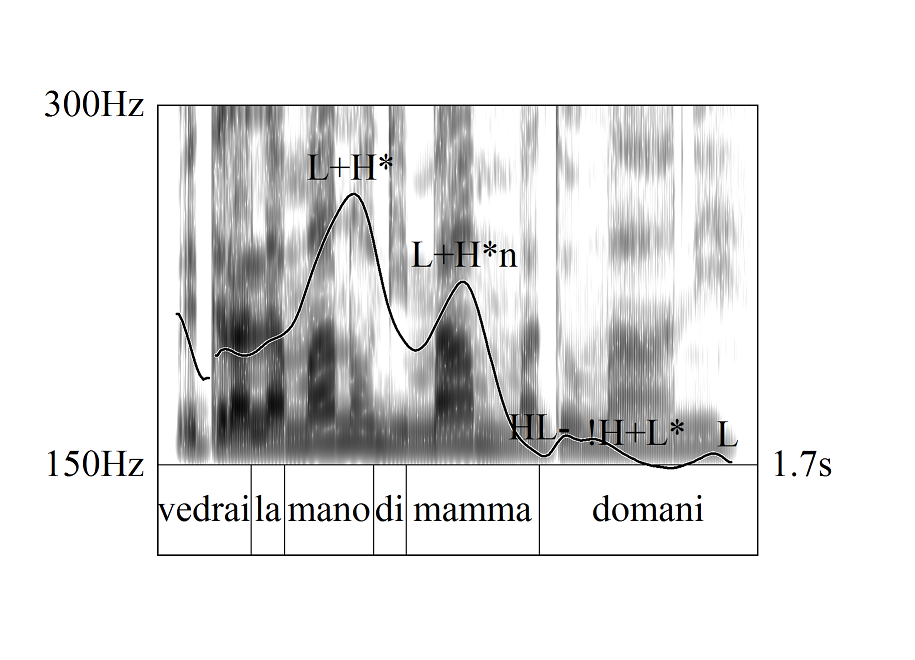
\includegraphics{images/102.png}}
\caption{The constituent medial fall analyzed as the L component of the narrow focus L+H* accent in Neapolitan. \textit{Vedrai la [MAno di MAMma] domani} `You'll see [Mom's hand] tomorrow)'. From Grice et al. (2005), Figure 13.1, original caption.}
\label{fig102}\end{figure}

\begin{figure}
\centering
\resizebox{\linewidth}{!}{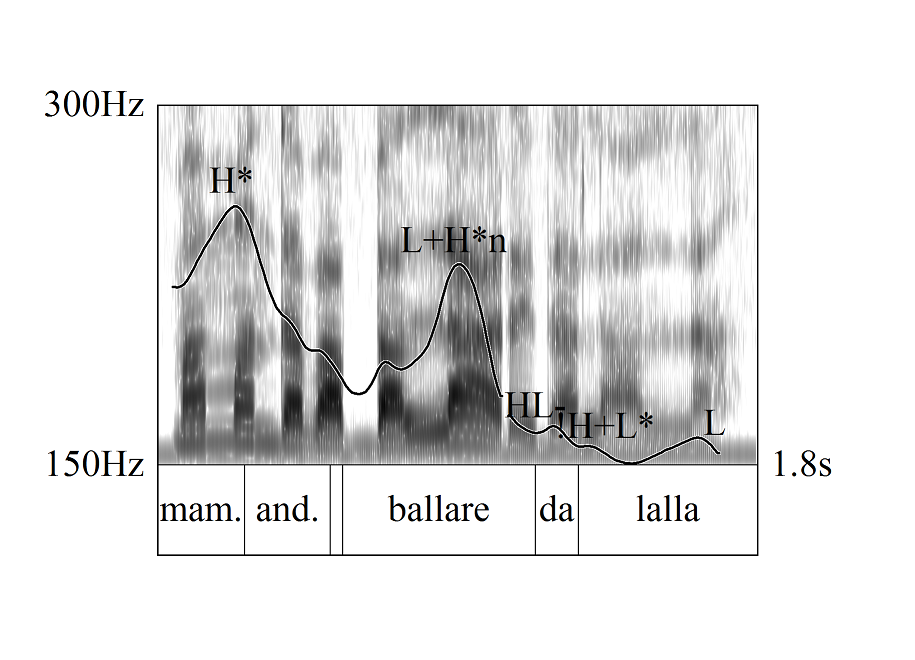
\includegraphics{images/103.png}}
\caption{Neapolitan: \textit{MAMma andava a [balLAre] da Lalla} `Mom used to go to [dance] at Lalla's'). Narrow focus declarative with L+H*. From Grice et al. (2005), Figure 13.7, original caption.}
\label{fig103}\end{figure}

As this quick survey shows, phonological descriptions of NI intonation are undergoing constant refinement, and a truly comprehensive account is still work in progress. Nevertheless, the knowledge available in the literature on some specific contrasts can serve as a useful starting point for our exploration of prosodic detail in NI. For the experimental chapters directly concerned with intonation (see Section~\ref{sec132}), the relevant introductory sections (Sections~\ref{sec212} and ~\ref{sec311}, respectively) will provide more detail about the AM accounts of the contrasts under examination.

\section{Structure of this book}\label{sec13}
Our exploration of how the AM framework deals with prosodic detail in NI will rely on four experimental studies of increasing complexity. These will be presented individually in the four next chapters (Sections~\ref{sec2}--\ref{sec5}) and discussed jointly in the concluding chapter (Section~\ref{sec6}). The four experimental chapters can be arranged monodimensionally, that is in a sequence, in the sense that the findings of the last constitute the input for the next. However, they can also be organized bidimensionally, that is as cells in a cross tabulation (see Table~\ref{tab11}).

\begin{table}[h]
\centering
\begin{tabular}{c c c}
\mytoprule
& Production & Perception\\
\midrule
Intonation & §~\ref{sec2} & §~\ref{sec3}\\
Tempo & §~\ref{sec4} & §~\ref{sec5}\\
\mybottomrule
\end{tabular}
\caption{Overview of the experimental chapters.}
\label{tab11}\end{table}

As we said above (Section~\ref{sec112}), we conceive prosodic detail as systematically \textit{produced and perceived} phonetic information cueing post-lexical contrasts and excluded from present \textit{abstractionist} accounts of prosody. Thus, as for the first dimension of the cross tabulation, prosodic detail must prove relevant in both \textit{production} (Sections~\ref{sec2}2 and ~\ref{sec4}) and \textit{perception} (Sections~\ref{sec3} and ~\ref{sec5}; see Section~\ref{sec131}). The second dimension deals with the phonetic dimensions which undergo information reduction in the framework we chose. As we said above (see Section~\ref{sec122}), in the AM framework phonetic information is pruned twice: first, by concentrating on \textit{f0} contours among the various suprasegmental cues (such as duration, amplitude, spectral tilt, and segmental reduction), and second, by reducing continuous modulations in \textit{f0} contours to sequence of frequency-time coordinates. Our experiments will address both kind of reductions (see Section~\ref{sec132}): we start by testing whether there is systematically produced and perceived phonetic detail which is not captured by the discretization of f0 contours into relevant events and predictable transitions (Sections~\ref{sec2}--\ref{sec3}; \textit{intonation} in Table~\ref{tab11}). Then we test whether other phonetic information on dimensions other than \textit{f0} is consistently produced and perceived, focussing in particular on the role of duration (Sections~\ref{sec4}--\ref{sec5}; \textit{tempo} in Table~\ref{tab11}) for the reasons we discuss in Sections~\ref{sec132} and~\ref{sec4}. In the rest of the book, the phrases melodic detail and temporal detail will be used to refer to phonetic detail at the prosodic level relating to the intonational and temporal dimensions, respectively, and instantiated acoustically by patterns in \textit{f0} and in duration of linguistic units.

Before turning to the experimental chapters, we comment on some of the methodological choices overarching individual experiments, by grouping them along the two dimensions of the cross tabulations discussed above (Sections~\ref{sec131}--\ref{sec132}), and by providing some brief information on the functional contrasts used in the experiments (Section~\ref{sec133}). The experiments will be followed by a final section in which we summarize our findings (Section~\ref{sec61}) and group our methodological innovations (Section~\ref{sec62}) before concluding on prosodic detail and exemplar-based approaches (Section~\ref{sec63}).

\subsection{Production and perception}\label{sec131}
The first remark to be made on the experimental chapters bearing on the acoustic manifestation of prosodic detail\footnote{Or on its \textit{production}, as said commonly (but perhaps in a not entirely correct way).} is on the nature of the speech material collected and analyzed. While research on phonetic detail in production has used material ranging from highly controlled scripted speech to spontaneous enacted conversations \citep{beckman1997typology}, we chose to focus exclusively on read speech. 

We agree with \citet{gilifivela2008intonation}, who points out that controlled and casual speech should both be used in the study of prosody, and that each should complement the other by providing both prospective insights and retrospective validations. Such a virtuous circle, however, could not be set in motion on the study of both production and perception of both melodic and temporal detail without exceeding the frame of a short monography. Our use of read controlled speech should be considered as a mere first step in the exploration of prosodic detail.

As for the evaluation of the perceptual role of prosodic detail, the motivation of our methodological choices require perhaps more elaboration. First, even researchers devoting great efforts to the exploration of phonetic detail\is{phonetic detail} acknowledge that ``we do not always use available phonetic detail'': listeners rather learn about it ``when it does not contradict other important cues to communicating meaning'' and use it ``when it is relevant to the task at hand'' \cite[9]{hawkins2011phonetic}. In this context, research striving to prove the importance of phonetic detail has to find the right task and the right cue interaction in order to maximize its visibility. Commenting on this line of research, \citet[8]{nguyen2009dynamical} say that ``the goal of current research on FPD is to show that FPD \textit{is} important in speech perception'' (original emphasis). As we stated above, our research interests bear on information reduction in phonological accounts of intonation. That is, we are rather interested in \textit{whether} phonetic detail is important in speech perception. Nevertheless, in our perception experiments we will try to maximize the impact of prosodic detail, by suppressing other cues usually available to listeners. It is known for example that indexical variation has a stronger effect in the perception of degraded speech, as in the case of low-pass filtered material \citep{church1994perceptual}. In our experiments, this will be achieved by using either excised (Section~\ref{sec3}) or resynthesized (Section~\ref{sec5}) stimuli.

The experimental tasks used in research on phonetic detail range from identification \citep{west1999perception} to word monitoring or word-spotting \citep{smith2000allophonic}, lexical decision \citep{hawkins2003effects} and sentence completion \citep{heinrich2010influence}. Given the pragmatic and informational nature of the functional contrasts involved in our manipulations, word monitoring and lexical decision could not be used. \citet{heinrich2010influence} used sentence completion in order to evaluate the intelligibility of speech in adverse listening conditions and, in turn, the role of r-resonances in building perceptual coherence. That is, the task did not deal with any functional contrast at all. For this reason, the core of our perceptual evaluations will be two-alternative forced-choice identification tasks.

\subsection{Intonation and tempo}\label{sec132}
As for information reduction, our experiments will concentrate on the phonological dimensions of intonation (Sections~\ref{sec2}--\ref{sec3}) and tempo (Sections~\ref{sec4}--\ref{sec5}). In the first two experiment we will address the reduction of phonetic information relative to fundamental frequency into a discretized string of tonal events, phonetically realized as coordinates along the \textit{f0} and time axes. In an investigation of prosodic detail, this is the natural place to start, since in AM phonetic information relative to transitions between the tonal events is considered as phonologically irrelevant, and derivable by interpolation rules. 

Sections~\ref{sec4} and ~\ref{sec5} deal with information reduction on a higher level. After dealing with detail along a phonetic dimension which is already taken into account in AM (namely \textit{f0} contours) in the first two experimental chapters, we will shift our attention to phonetic dimensions which are altogether absent in phonological representations bridging phonetic substance and post-lexical meaning. Among these potentially interesting prosodic cues, namely duration, amplitude, \citep{shattuck1996prosody} spectral tilt and measures of segmental reduction \citep{ladd2008intonational} and voice quality \citep{campbell2003voice}, we decided to focus on duration. This is because its effects on post-lexical meaning have been more widely studied (see Section~\ref{sec41}), and it is more reliably investigated using acoustic data alone, that is the only kind of data which could be collected in our fieldwork sessions in Naples.

The relevant chapters will provide an extensive motivation of our terminological choices (see Section~\ref{sec4} and especially Section~\ref{sec511}), but for the sake of clarity we can anticipate some remarks of our use of duration, tempo, and durational and temporal patterns. We use \textit{duration} in its fairly uncontroversial sense of an acoustic propriety of linguistic units, which can be measured in an absolute way along the time dimension and is usually expressed in milliseconds. However, since ``it is not the duration of a single segment but the complex relationships between segment durations that convey information to the listener'' \citep{lyberg1981observations}, we use \textit{durational patterns} when referring to vectors grouping duration of sub-units inside an overarching unit, as for example in the case of phones within an utterance. In this case, of course, measures can be both absolute and relative to the duration of the overarching unit.

Our use of \textit{tempo}\is{tempo}, on the other hand, requires some elaboration. Already in the 1970s, \citet{wood1973speech} remarked that terminology in this area was quite uncertain, and that ``tempo is not one single, unambiguous concept''. However, it is clear that in his account tempo belongs to the conceptual family of measures such as speech rate, rate-of-speech, rate of speech production, speed of talking, talking rate or speaking tempo. Tempo had this meaning since at least \citet{abercrombie1967elements}, according to which ``tempo (speed of speaking) is best measured by rate of syllable succession'', and is nowadays prevalently used in this sense (e.g. \citealt{trouvain2004tempo}). However, tempo has also been used in another sense which is more adapted to our research interests, notably by \citet{lehiste1970suprasegmentals}. In her account of suprasegmental phonetic features and their linguistic function, tempo is seen as the formal dimension bridging durational phonetic information with post-lexical meaning. In this sense, tempo can be contrasted to both intonation (which deals with phonetic information relative to \textit{f0} contours rather than duration) and length (which deals with lexical rather than post-lexical meaning). In the following, tempo will be used in this particular meaning of a formal phonological dimension which is parallel to intonation, rather than in the more widespread phonetic interpretation consistent for example with Abercrombie's use. It is important to note that this terminological choice seems to entail a particular vision of prosody, in which the temporal dimension is seen as parallel to the intonational one. We stress that we do not commit to this interpretation, and we rather take it as a working hypothesis, which we will actually test in Section~\ref{sec5}. That is, we take tempo to design a phonological dimension in order to have the terminological support to formulate the claim that durational differences are phonologically relevant.

As a result, the phrase \textit{temporal patterns} will be used when referring to phonological accounts of phonetic durational patterns spanning over the utterance. In this respect, temporal patterns can be seen as the temporal equivalent of what tunes represent in intonation, namely formal structures which combine primitives into a larger domain. As we said above, however, these terminological choices will be discussed at greater length in the introductory pages of the relevant experimental chapters.

\subsection{Sentence modality contrasts}\label{sec133}\is{sentence modality}
Given that our understanding of phonetic detail emphasizes, rather than speaker-specific variation, language-specific variation and thus allophonic detail in its broadest sense (see Section~\ref{sec112}), our research on prosodic detail will be based on functional contrasts at the post-lexical level. The majority of our experiments (Sections~\ref{sec4}, ~\ref{sec5} and ~\ref{sec33}) will use sentence modality contrasts. \citet{sadock1985speech} call \textit{sentence type} the ``coincidence of grammatical structure and conventional conversational use''. By grammatical structures they mean not only specific syntactic constructions, but also ``special particles, affixes, word order, intonations, missing elements, or even phonological alterations''. The inventory of the possible conventional conversational uses is also very broad, and ranges from making a bet to asking for information or to ordering someone to do something \citep{lyons1977semantics}. By examining pairs of grammatical structures and conversational uses in 23 languages, \citet{sadock1985speech} provide a tentative taxonomy of apparently universal sentence types, grouped in the three macro-classes of declaratives, imperatives and interrogatives.  In the following years, the phrase \textit{sentence modality} has been extensively used in prosodic research focussing on a particular contrast between sentence types, namely the one between declaratives and interrogatives which are distinguished through prosody alone. For languages such as Italian, this is the case of the opposition between statements and yes-no questions,\footnote{For languages such as English or French, in which statements and yes-no questions can have different morphosyntactic structures, sentence modality contrasts rather oppose statements and so-called ``declarative questions''.} as seen above (Section~\ref{sec121}).

Sentence modality contrasts have a sort of privileged status in prosodic research. They have always drawn consistent attention, even before the development of phonological approaches to intonation (\citealt{kretschmer1938ursprung}, among others), because of the immediacy and the relevance of the functional contrast involved. Other post-lexical functional contrasts expressed by prosody, as in the case of information packaging, are less self-evident and more theory-dependent. That is, whereas segmental phonology is based on lexical contrastiveness, which does not need to be theorized in order to be tested (i.e. lexical contrast is somehow accessible to the epilinguistic conscience of the speaker/listener), research on intonation focusses on the link between prosodic acoustic cues and post-lexical meaning which apparently needs to be structured in a linguistic theory (e.g. sentence semantics, pragmatics, information structure). We will comment on this later on (see Section~\ref{sec243}); for the sake of the present discussion, it is only necessary to say that sentence modality contrasts were used in the majority of the experimental work presented here precisely for this reason. That is, since the investigation of prosodic detail already entails, by definition, the exploration of previously unaccounted phonetic information, we decided at least to concentrate on the most thoroughly accounted functional contrast \citep{huddleston1994contrast,haan2002speaking}.

The only exception to this general methodological choice is represented by the exploration of the contrast between narrow focus yes-no questions and partial topic statements in Sections~\ref{sec2} and~\ref{sec32}. Details on the functional aspects of this contrast will be provided in the relevant introductory sections (see especially Section~\ref{sec212}). With respect to the present discussion, the motivation for this choice lies in the extreme substantial (phonetic) similarity between the two contexts, which is in itself an ideal starting point for the exploration of dissimilarities in phonetic detail.